%Chapter 4

\chapter{Application} % Main chapter title

\lhead{Chapitre 4. \emph{Application}}

\section{Introduction}
	
	Nous allons aborder dans ce chapitre les détails techniques de notre implémentation (langage de programmation, Frameworks, etc.), ensuite nous présenterons l'interface que nous avons conçu pour l'application de notre approche. Enfin, nous examinerons plus en détail certains exemples et résultats de recherches d'images.

\section{Outils utilisés}

	La configuration de la machine utilisée est comme suit : Processeur Intel R Core TM i7-2670QM CPU @ 2.20GHz , système d’exploitation GNU/Linux - Ubuntu 14.04 x64.

	Nous avons implémenté nos approches avec le langage de programmation Python, version 3.0 et à l'aide de différents Framework et bibliothèques.

	Pour développer l'interface graphique de notre implémentation, nous avons utilisé PyQt4, un module pour python qui permet de le lier à la librairie Qt (framework pour le développement d'applications multi-plate-formes).

\subsection{Le langage Python}
	Nous avons choisi ce langage pour différentes raisons dont nous citons:

\begin{itemize}

\item Une facilité d’écriture et de compréhension du code.
\item Son niveau d'abstraction permet de mettre en place des prototypes et de les tester rapidement
\item Sa syntaxe organisée, l'indentation obligatoire rend le code trivialement lisible.
\item Un grand nombre de bibliothèques puissantes.
\item Une documentation très variée.
\item Une grande communauté qui permet d'obtenir de l'aide rapidement.
\end{itemize}


\subsection{Theano}
	Theano est un framework en Python très utilisé, il est l'un des plus anciens aussi et du coup, beaucoup de recherches se sont basées dessus. 

	Il a été conçu par le laboratoire MILA (Montréal Institute for Learning Algorithms) de l’Université de Montréal. C'est un projet Open Source que de nombreux autre chercheurs de différents laboratoires et institutions ont fini par rejoindre (Google Deepmind, New  York  University, NVIDIA Corporate, Meiji  University Tokyo ..etc ) [Theano 16].

	Ce framework permet de définir des expressions mathématiques symboliques en les représentant par des graphes orientés acycliques. Ces derniers sont constitués de deux types de nœuds: \textbf{Variable} qui représente les données et \textbf{Appliquer} qui représentes les opérations mathématiques. Cette représentation permet une manipulation simple des expressions et fonctions mathématiques dont, entre autre, la génération automatique de leurs dérivées.\\

Par exemple, soit un "scalar" x: \\

>> \textit{x = theano.tensor.dscalar('x')}\\

ensuite on définit une expression, la fonction carré par exemple: \\

>> \textit{y = x ** 2}\\

	On peut aussi visualiser le graphe généré qui résume toute la fonction, avec la ligne suivante:\\

>> \textit{theano.printing.pydotprint(y, outfile="yGraph.png", var\_with\_name\_simple=True)}\\

On aura comme résultat le graphe de la figure (Figure 4.1) ci-dessous:

\begin{figure}[H]
	\centering
		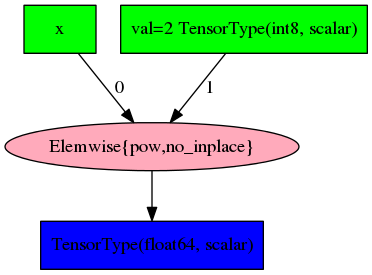
\includegraphics[width=3in]{Figures/yGraph.png}
	\caption[TheanoGraph]{Visualisation du graphe d'une fonction}
	\label{fig:Electron}
\end{figure}

	Les nœuds en verts sont les arguments de l'opérateur puissance (pow) qui est en bleu, et le résultat est dans le nœud en rose.
	Rappelons que lors de la phase d'apprentissage des réseaux de neurones (perceptrons multicouches et autres), il est nécessaire lors de la rétro-propagation du gradient de calculer des dérivés en fonctions de plusieurs paramètres. Theano nous facilite cela puis-que les dérivations s'effectuent simplement en appliquant la fonction \textit{grad}. 
Donc, la dérivée de la fonction \textbf{y} que nous avons définie, par rapport à \textbf{x} peut être calculer comme suit: \\

>> \textit{gy = T.grad(y, x)}\\

\textbf{gy} contient dorénavant la dérivée de \textbf{y} par rapport à \textit{x}, qui n'est rien d'autre que $2*x$ .\\

%>> \textit{theano.pp(gy)}\\
% '((fill((x ** TensorConstant{2}), TensorConstant{1.0}) * TensorConstant{2}) * (x ** (TensorConstant{2} - TensorConstant{1})))'\\
 
	En essayant d'afficher le graphe de \textbf{gy} nous obtenons la figure (Figure 4.2) ci-dessous:

\begin{figure}[H]
	\centering
		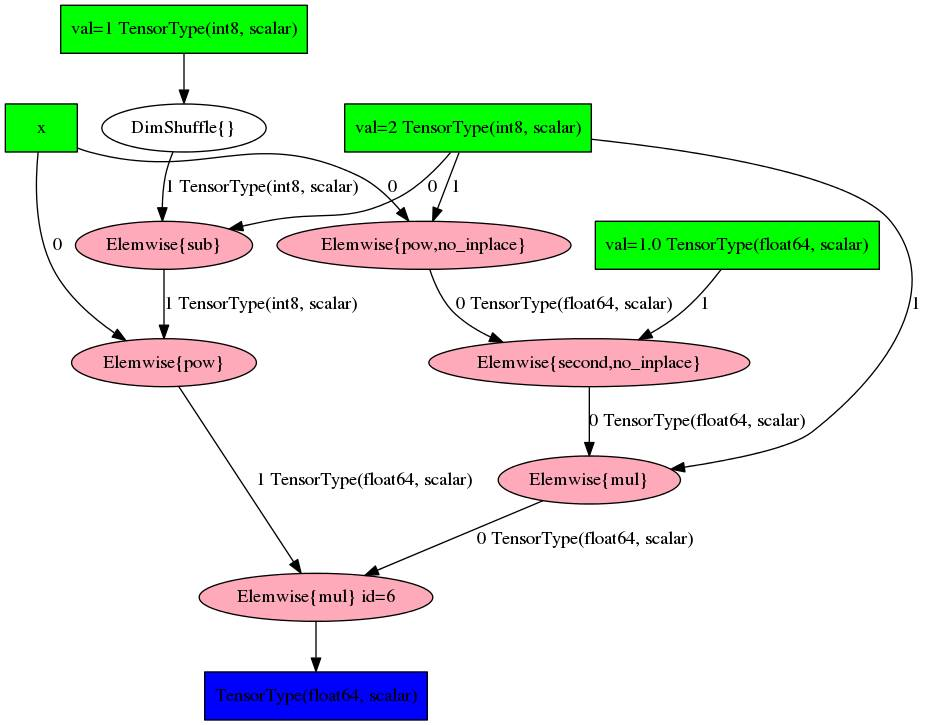
\includegraphics[width=5in]{Figures/beforeOptimization.png}
	\caption[TheanoGraph]{Visualisation du graphe de \textbf{gy} avant optimisation.}
	\label{fig:Electron}
\end{figure}

	Ce graphe n'est pas évident à comprendre alors qu'il s'agit seulement de la fonction $ gy = 2*x$. Compiler le graphe de \textbf{gy} à l'aide de la fonction "function" de Theano pour le rendre exécutable s'effectue comme suit:\\

>> \textit{f = theano.function([x], gy)}\\

	Cette opération optimise le calcul de \textbf{gy}, et le graphe de \textbf{f} devient comme le montre la figure ci-dessous:

\begin{figure}[H]
	\centering
		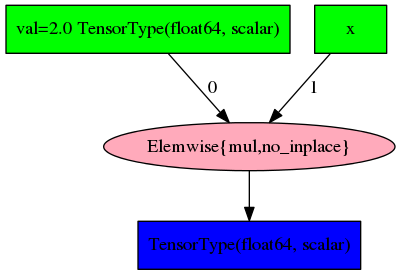
\includegraphics[width=3in]{Figures/afterOptimization.png}
	\caption[TheanoGraph]{Visualisation du graphe de \textbf{gy} après optimisation.}
	\label{fig:Electron}
\end{figure}

	Ceci montre à quel point Theano est puissant dans sa gestion des fonctions et de leurs dérivées, ainsi que leurs optimisations en quelques lignes de codes.
	
	Une notion très importante qui existe dans Theano est celle des \textit{variables symboliques}. Elle peuvent être considérées comme des tampons (buffers) qui contiennent des valeurs qui peuvent être partagées entre plusieurs fonctions de Theano.\\

	Un autre point fort de Theano est l'optimisation pour l'utilisation de matrices multi-dimensionnelles, mais aussi la facilité de compiler et exécuter les opérations sur des GPU au lieu des CPU.\\

	Theano fut suivi par d'autres frameworks qui ont repris les mêmes principes, les plus connus sont Tensorflow de Google, Blocks, Lasagne.

\subsection{Autres Frameworks}
	Pour ce familiariser avec Theano, il existe d'autres frameworks qui ajoutent des couches d'abstraction à Theano pour faciliter son utilisation, comme Blocks, Lasagne et Keras.
	Le modèle VGG-CNN-S du réseau à convolution que nous avons utilisé dans notre algorithme est implémenté en Lasagne après avoir été converti de Caffe (Caffe étant un autre Framework en C++ développé par le laboratoire Berkeley Vision and Learning Center).\\

	Pour implémenter les autoencoders de nos approches, nous avons utilisé Blocks [Mer et al. 15], c'est un framework de theano qui facilite la définition de modèles et leur modifications. Il introduit des outils pour l'apprentissage, la visualisation et la sérialisation. Enfin, le framework Fuel [Mer et al. 15] permet de formater les données d'apprentissage d'une façon qui facilite leur manipulation, surtout quand les tailles de ces dernières deviennent importantes.\\

	Dans notre cas, au lieu de le définir couche par couche, l'Autoencoder 4x1x4 est défini simplement par:\\

>> \textit{ae = MLP([Tanh(), Tanh()], [4096, 1000, 4096],
              weights\_init=IsotropicGaussian(0.01),
              biases\_init=Constant(0))\\
   }           

Puis, il est initialisé par:\\

>> ae.initialize()\\

	Ces deux frameworks sont développés aussi par le laboratoire MILA, ils forment une base solide pour le développement d’approches basées sur l'apprentissage profond.

\section{Interface de l'application}

	Après notre étude comparative dans le chapitre précédent entre les différentes approches que nous avons réalisées, nous avons décidé d'implémenter dans l'interface graphique la meilleure approche (celle qui a donné les meilleures mesures de performance), qui est celle du Denoising Autoencoder 4x1x4.

	L'interface que nous avons développée (Figure 4.3) pour l'implémentation de notre approche permet de sélectionner une base d'images qui servira de recueil pour les résultats des requêtes, comme le montre la figure (Figure 4.3).


\begin{figure}[H]
	\centering
		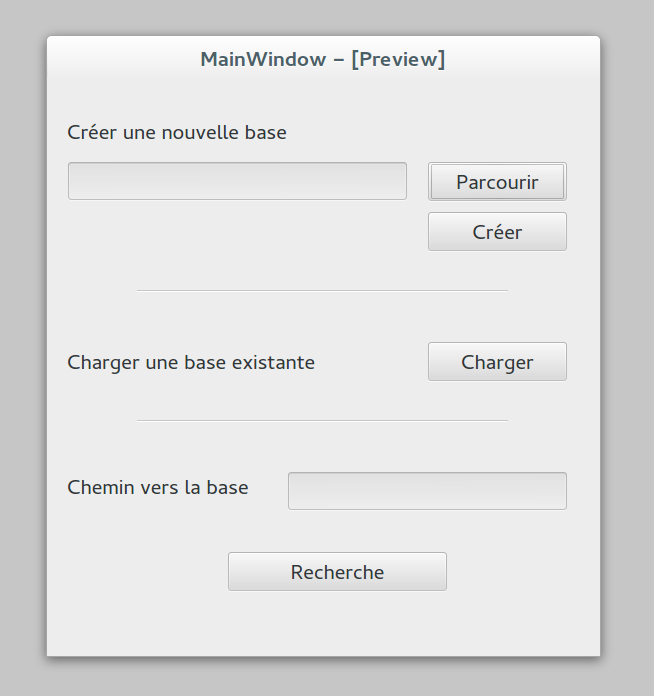
\includegraphics[width=3in]{Figures/mainMenu.png}
	\caption[Menu principal]{Menu principal.}
	\label{fig:Electron}
\end{figure}

	Nous pouvons choisir de créer une nouvelle base, pour cela on doit indiquer le lien vers le dossier contenant la base d'images, puis appuyer sur le bouton \textit{Créer}. Le programme dans ce cas va créer la description de chaque image en la faisant passer par le réseau à convolution, ensuite extraire la description sémantique de l'image de la couche 4096b et finalement créer la description compressée en utilisant le Denoising Autoencoder 4x1x4.
	C'est cette description qui sera enregistrée en tant que modèle pour la recherche d'images. On peut aussi charger une base déjà existante en appuyant sur le bouton \textit{Charger}.

	En cliquant sur le bouton \textit{Recherche}, une nouvelle fenêtre s'ouvre qui permet de sélectionner une image qui fera office de requête (Figure 4.4). Une fois l'image sélectionnée, le programme va créer sa représentation sémantique compressée. Le bouton \textit{Chercher} lance la recherche et affiche les cinq images jugées les plus ressemblantes (top-5).

\begin{figure}[H]
	\centering
		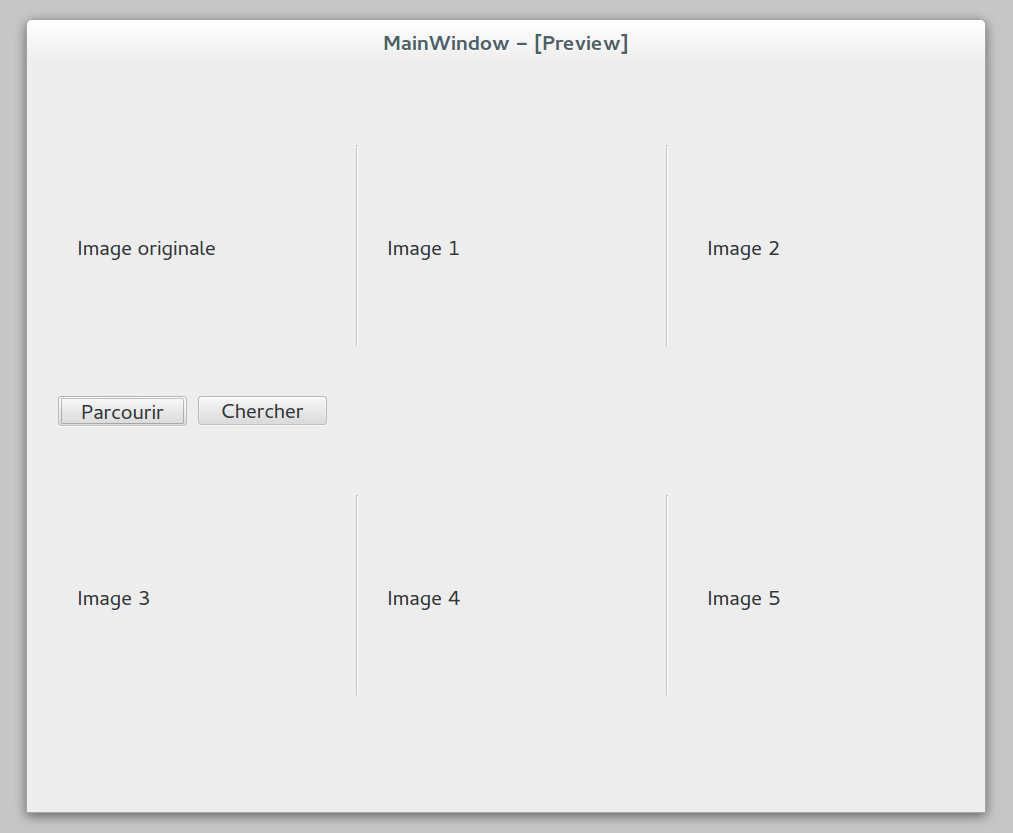
\includegraphics[width=4.5in]{Figures/search.png}
	\caption[]{Interface de recherche d'images.}
	\label{fig:Electron}
\end{figure}

\section{Tests}

	Nous allons dans cette partie faire quelques tests de notre système de recherche d'images par le contenu. Les deux figures (Figure 4.6) et (Figure 4.7) ci-dessous, représentent deux tests effectués sur deux images prises respectivement des deux bases d'images \textbf{WANG} [Wan et al.,01][Li et Wan.,03] et \textbf{Caltech-101} [Fei et al. 04].
	
\begin{figure}[H]
	\centering
		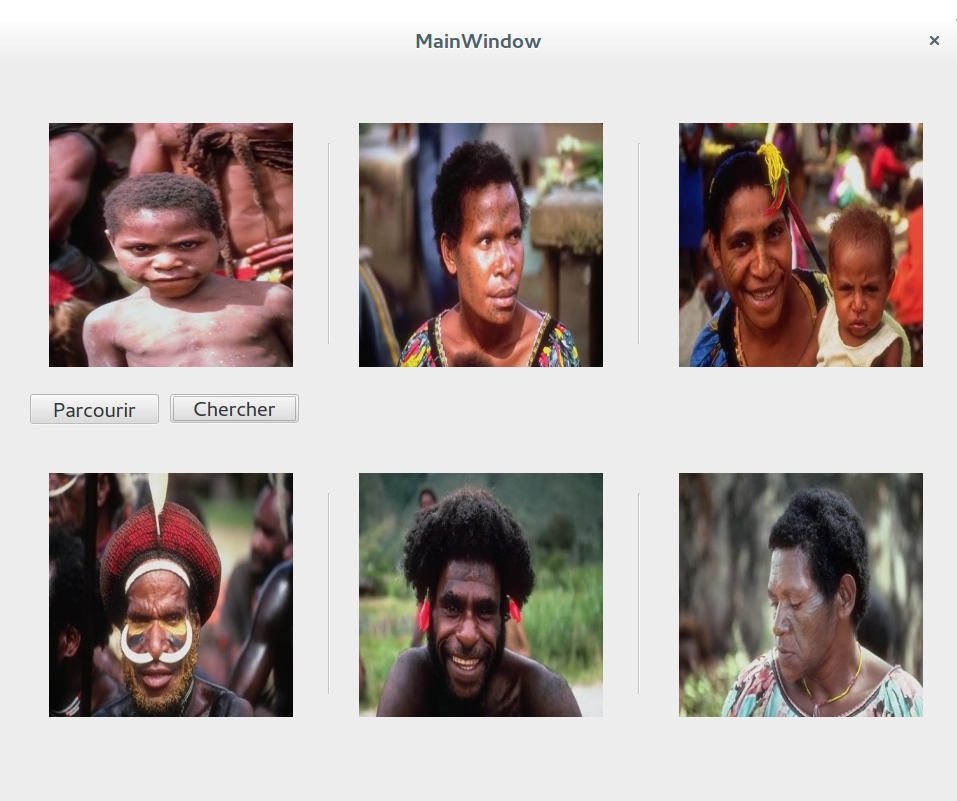
\includegraphics[width=4in]{Figures/guiTests1.png}
	\caption[]{Résultat de recherche d'une image de la base WANG.}
	\label{fig:Electron}
\end{figure}

\begin{figure}[H]
	\centering
		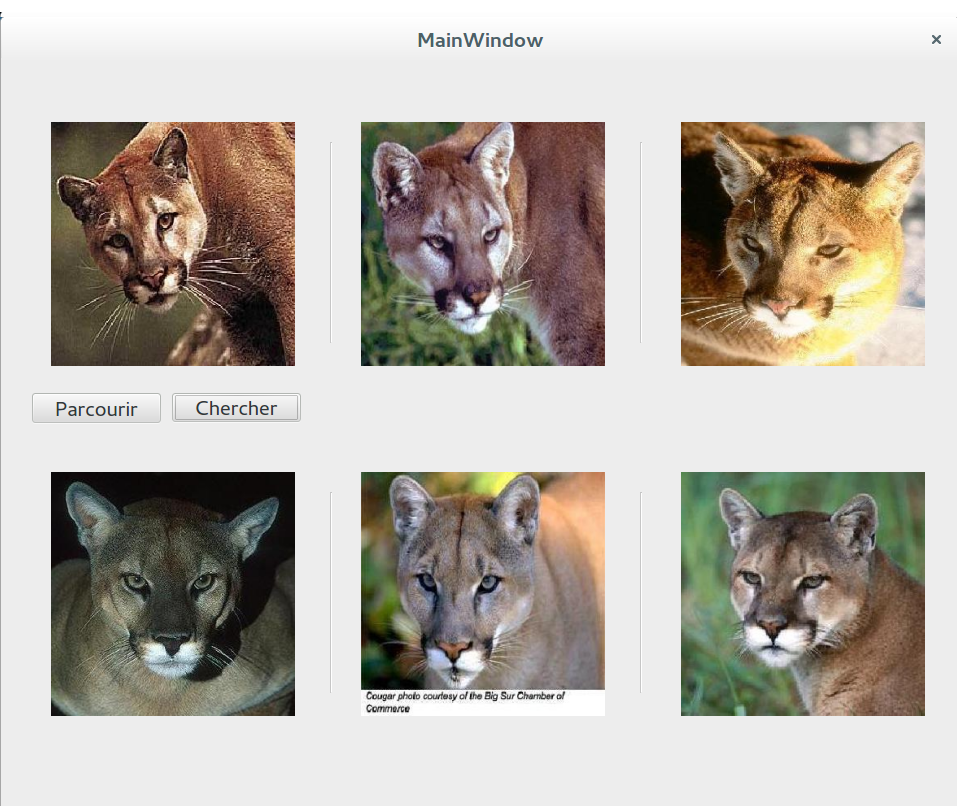
\includegraphics[width=4in]{Figures/guiTests2.png}
	\caption[]{Résultat de recherche d'une image de la base Caltech-101.}
	\label{fig:Electron}
\end{figure}


	L'image prise de le base WANG appartient à la classe \textit{Africans}, et celle de Caltech-101 à la classe \textit{Cougar\_face}. Nous pouvons très bien voir la qualité des résultats obtenus sur le top-5 des images retournées.
	
	Ces deux classes donnent de bons taux en terme de performance. Nous allons maintenant donner un exemple d'une image de la base Caltech-101 de la classe \textit{Crab}, qui ne donne pas d'aussi bons résultats. La figure suivante (Figure 4.8) montre le top-20 (de gauche à droite, de haut en bas) des images retournées par notre système:

\begin{figure}[H]
\begin{tabular}{ccccc}\\


\multicolumn{5}{c}{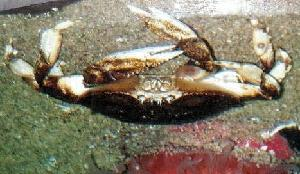
\includegraphics[width=9cm]{Figures/crab/0.jpg}}\\
\multicolumn{5}{c}{Image requête de la classe \textit{Crab}}\\
%\hline
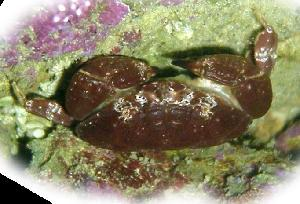
\includegraphics[width=3cm]{Figures/crab/1.jpg}
&
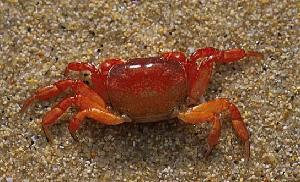
\includegraphics[width=3cm]{Figures/crab/2.jpg}
&
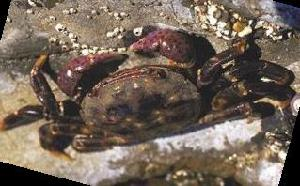
\includegraphics[width=3cm]{Figures/crab/3.jpg}
&
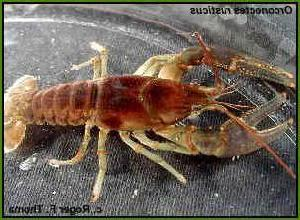
\includegraphics[width=3cm]{Figures/crab/4.jpg}
&
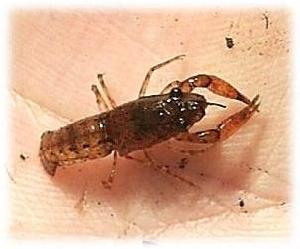
\includegraphics[width=3cm]{Figures/crab/5.jpg}\\
Crab & Crab & Crab & Crayfish & Crayfish\\


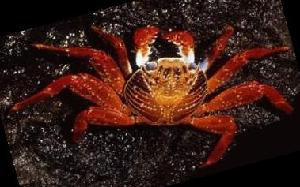
\includegraphics[width=3cm]{Figures/crab/6.jpg}
&
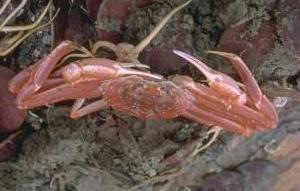
\includegraphics[width=3cm]{Figures/crab/7.jpg}
&
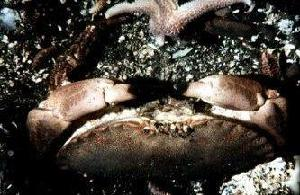
\includegraphics[width=3cm]{Figures/crab/8.jpg}
&
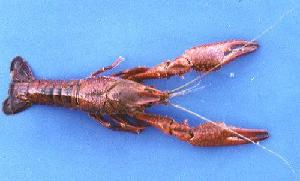
\includegraphics[width=3cm]{Figures/crab/9.jpg}
&
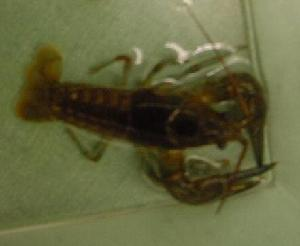
\includegraphics[width=3cm]{Figures/crab/10.jpg}\\
Crab & Crab & Crab & Crayfish & Crayfish\\


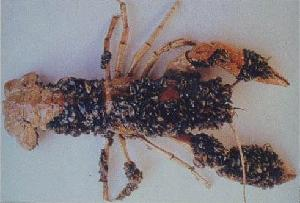
\includegraphics[width=3cm]{Figures/crab/11.jpg}
&
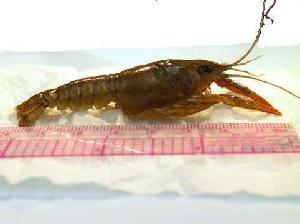
\includegraphics[width=3cm]{Figures/crab/12.jpg}
&
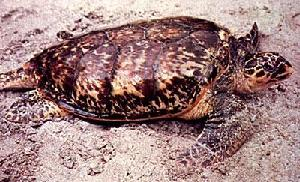
\includegraphics[width=3cm]{Figures/crab/13.jpg}
&
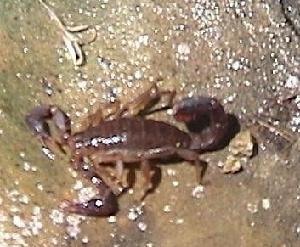
\includegraphics[width=3cm]{Figures/crab/14.jpg}
&
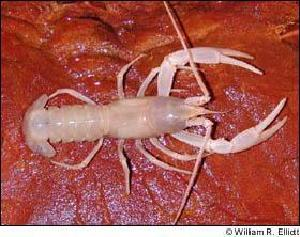
\includegraphics[width=3cm]{Figures/crab/15.jpg}\\
Crayfish & Crayfish & Hawksbill & Scorpion & Crayfish\\



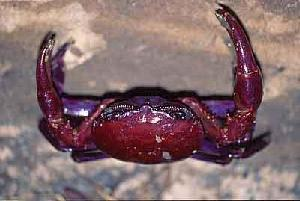
\includegraphics[width=3cm]{Figures/crab/16.jpg}
&
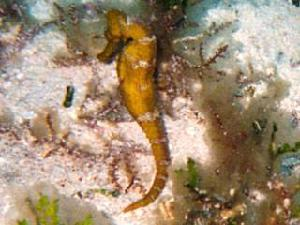
\includegraphics[width=3cm]{Figures/crab/17.jpg}
&
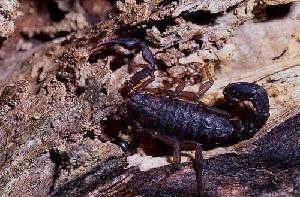
\includegraphics[width=3cm]{Figures/crab/18.jpg}
&
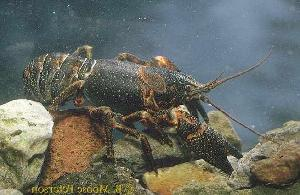
\includegraphics[width=3cm]{Figures/crab/19.jpg}
&
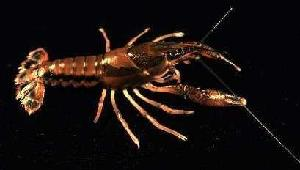
\includegraphics[width=3cm]{Figures/crab/20.jpg}\\
Crab & Sea\_horse & Scorpion & Crayfish & Crayfish\\

\end{tabular}
\caption[comp7]{Résultats obtenus sur l'image d'un Crabe.}
\end{figure}

	Les mesures de performance pour une image comme celle-ci ne sont pas assez bonnes. Le top-1, top-5 et top-10 des images retrournées sont acceptables, mais si on cherche encore plus de résultats, le système n'arrive pas à donner de meilleurs résultats. N’empêche que les images non pertinentes (qui n'appartiennent pas à la classe \textit{Crab}) ne sont pas vraiment loin du concept d'animal marin ou de crustacé, cela est possible grâce aux descriptions sémantiques des images.
	
	Nous allons présenter cette fois-ci d'autres tests sur la base WANG (Figure 4.9) et Caltech-101 (Figure 4.10), qui ne donnent pas de bons résultats mais les images retournées ne sont pas forcément de contenu différent.
	
\begin{figure}[H]
\begin{tabular}{ccccc}\\


\multicolumn{5}{c}{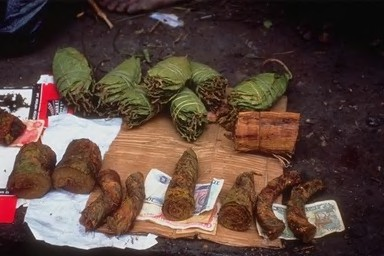
\includegraphics[width=6cm]{Figures/africans/0.jpg}}\\
\multicolumn{5}{c}{Image requête de la classe \textit{Africans}}\\
%\hline


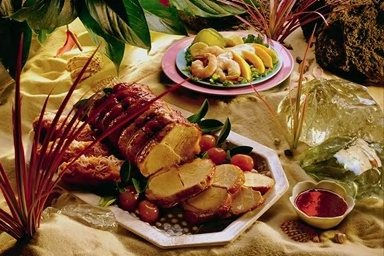
\includegraphics[width=3cm]{Figures/africans/1.jpg}
&
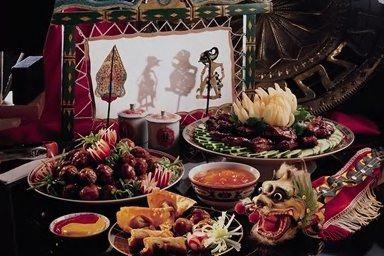
\includegraphics[width=3cm]{Figures/africans/2.jpg}
&
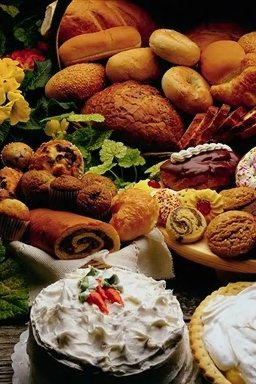
\includegraphics[height=2cm,width=3cm]{Figures/africans/3.jpg}
&
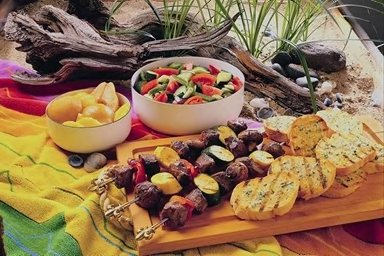
\includegraphics[width=3cm]{Figures/africans/4.jpg}
&
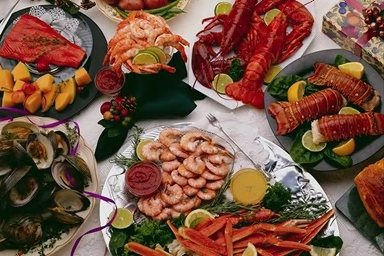
\includegraphics[width=3cm]{Figures/africans/5.jpg}\\
Foods & Foods & Foods & Foods & Foods\\

\end{tabular}
\caption[comp7]{Résultats obtenus sur une image de la classe \textit{Africans}.}
\end{figure}

	Cette image requête donne des mesures de performance qui ne dépassent pas les 20\% de reconnaissance, le système est sensé trouver des images de la classe \textit{Africans} alors qu'il retourne à la place des images de la classe \textit{Foods}. Il est clair que cette image requête est bien différente des images de la classe \textit{Africans} qui contient des images du peuple Africain. Le contenu de cette image requête (nourriture ou bien médicament) est très proche du concept de la classe \textit{Foods}, le système donc retourne des images qui ont le même contenu mais qui ne sont pas de la même classe. Ce problème est dû au fait que les images de la base WANG appartiennent seulement à une seule classe.

\begin{figure}[H]
\begin{tabular}{ccccc}\\


\multicolumn{5}{c}{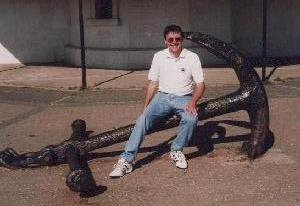
\includegraphics[width=6cm]{Figures/anchor/0.jpg}}\\
\multicolumn{5}{c}{Image requête de la classe \textit{Anchor}}\\
%\hline


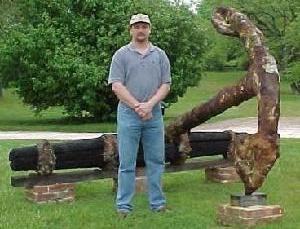
\includegraphics[width=3cm]{Figures/anchor/1.jpg}
&
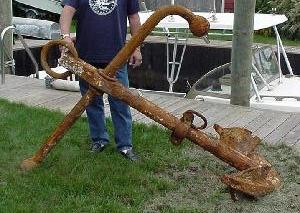
\includegraphics[width=3cm]{Figures/anchor/2.jpg}
&
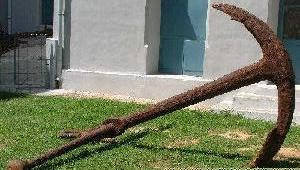
\includegraphics[width=3cm]{Figures/anchor/3.jpg}
&
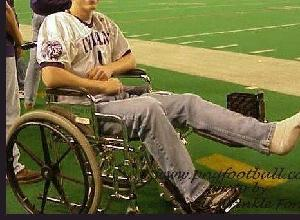
\includegraphics[width=3cm]{Figures/anchor/4.jpg}
&
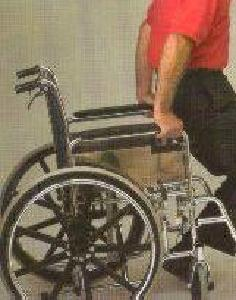
\includegraphics[height=2cm,width=3cm]{Figures/anchor/5.jpg}\\
Anchor & Anchor & Anchor & Wheelchair & Wheelchair\\

\end{tabular}
\caption[comp7]{Résultats obtenus sur une image de la classe \textit{Anchor}.}
\end{figure}

	Cette image requête de la base Caltech-101 appartient à la classe \textit{Anchor}, les 3 premières images (top-3) sont correctes, par contre la quatrième et la cinquième image ne le sont pas. On peut remarquer une similarité entre ces deux dernières avec l'image requête, on peut dire que le contenu (un homme qui s'assoit) est assez similaire.

\section{Conclusion}

	Nous concluons ce chapitre en mettant l'accent sur les avantages qu'apporte la représentation des mathématiques symboliques que propose le framework Theano. Il permet entre autre de faciliter la description de modèles complexes, mais aussi de faciliter la phase d'entraînement (la rétro-propagation) grâce au calcul automatique des dérivés.
	
	Nous avons ensuite montré des résultats de notre système de recherche d'images par le contenu sur différents exemples de requête, où nous avons pu observer ce que la représentation sémantique des images donne comme réponse.
	
	